\paragraph{QuizziPedia::Front-End::Services::Utils}

\label{QuizziPedia::Front-End::Services::Utils}
\begin{figure}[ht]
	\centering
	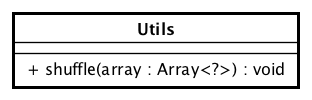
\includegraphics[scale=0.60]{UML/Classi/Front-End/QuizziPedia_Front-end_Services_Utils.png}
	\caption{QuizziPedia::Front-End::Services::Utils}
\end{figure}\FloatBarrier
\begin{itemize}
	\item \textbf{Descrizione}: rappresenta un oggetto contenente metodi che non appartengono a nessuna classe ma sono utili per svariati scopi.
	\item \textbf{Utilizzo}: utilizzata per varie funzionalità non appartenenti a nessuna classe in particolare;
	\item \textbf{Metodi}:
	\begin{itemize}
		\item \texttt{+} \texttt{shuffle(array: Array<>)} \\ Metodo che permette di mescolare in maniera casuale gli elementi di un array; \\
		\textbf{Parametri}:
		\begin{itemize}
			\item \texttt{array: Array<>} \\ Campo dati che contiene un array di elementi di qualsiasi tipo.
		\end{itemize}

	\end{itemize}
\end{itemize}
